\appendix

\section{Appendix Overview}
\label{sec:appendix}

This appendix provides additional methodological details and extended results complementing the main paper.

Appendix~\ref{sec:semantic_constraints} details the lightweight semantic constraints referenced in \S\ref{subsec:data-generation}, which \name{} can optionally enforce while instantiating the latent relational source to push it toward more plausible configurations.

Appendix~\ref{app:generating_non_rel} reports the main tests cited in \S\ref{sec:intro} that motivate \name{}. In particular, it shows that perturbed parallel and sequential questions are difficult to synthesize from existing relational tables, and that non-relationalization markedly degrades LLM performance in multi-table settings.

Appendix~\ref{sec:exp_train} reports the detailed experimental results underlying \S\ref{sec:discussion}, together with the finetuning configuration. It provides per-setting performance of all evaluated baselines on parallel and sequential questions over both relational and non-relational tables, as well as the training setup and data composition used in the finetuning experiments.

Appendix~\ref{sec:data_statistics} reports statistics on the \name{}-generated data used throughout the experiments, including the number of retained instances per experiment, the share of candidates discarded during generation, and how instances are balanced across table counts, aggregation operators, unit settings, and relational versus non-relational views.

Appendix~\ref{sec:prompts} illustrates the prompts used at each stage of \name{}, covering latent relational source generation, semantic constraint generation, natural-language question generation and verification for both parallel and sequential regimes, and the inference prompt given to the evaluated models.

Appendix~\ref{app:license} details the licenses of all artifacts used in this work, all of which permit research use.

\begin{table*}[t!]
\centering
\setlength{\tabcolsep}{0.15em}
\renewcommand{\arraystretch}{1.16}
\small{
\resizebox{\textwidth}{!}{
\begin{tabular}{lllccccccccccccccc}
\toprule
 &  &  & \multicolumn{3}{c}{\textit{2}} 
 & \multicolumn{3}{c}{\textit{3}} 
 & \multicolumn{3}{c}{\textit{5}} 
 & \multicolumn{3}{c}{\textit{10}} 
 & \multicolumn{3}{c}{\textit{20}} \\
\cmidrule(lr){4-6}
\cmidrule(lr){7-9}
\cmidrule(lr){10-12}
\cmidrule(lr){13-15}
\cmidrule(lr){16-18}
 &  & 
 & \texttt{com} & \texttt{quant} & \texttt{avg}
 & \texttt{com} & \texttt{quant} & \texttt{avg}
 & \texttt{com} & \texttt{quant} & \texttt{avg}
 & \texttt{com} & \texttt{quant} & \texttt{avg}
 & \texttt{com} & \texttt{quant} & \texttt{avg} \\ 
\midrule

\multirow{8}{*}{\rotatebox[origin=c]{90}{\texttt{environmental}}}
 & \multirow{4}{*}{\rotatebox[origin=c]{90}{\texttt{same unit}}}
 & \texttt{gpt-5-mini}
 & 94.74 & 89.47 & 92.11
 & 92.11 & 93.43 & 92.77
 & 95.45 & 89.19 & 92.32
 & 87.10 & 60.75 & 73.93
 & 87.88 & 21.21 & 54.55 \\
 &  & \texttt{Qwen3.5-122B}
 & 89.47 & 96.06 & 92.76
 & 97.37 & 89.47 & 93.42
 & 86.47 & 85.14 & 85.80
 & 80.56 & 70.84 & 75.70
 & 84.85 & 57.58 & 71.22 \\
 &  & \texttt{Qwen3.5-35B}
 & 86.84 & 86.84 & 86.84
 & 84.21 & 93.43 & 88.82
 & 89.19 & 82.44 & 85.81
 & 88.89 & 58.34 & 73.61
 & 78.79 & 36.36 & 57.58 \\
 &  & \texttt{Qwen3.5-9B}
 & 65.79 & 67.11 & 66.45
 & 65.79 & 67.11 & 66.45
 & 59.46 & 54.05 & 56.76
 & 52.78 & 33.33 & 43.06
 & 42.42 & 10.61 & 26.51 \\
\cmidrule(lr){2-18}
 & \multirow{4}{*}{\rotatebox[origin=c]{90}{\texttt{unit diff}}}
 & \texttt{gpt-5-mini}
 & 63.16 & 47.37 & 55.27
 & 42.11 & 34.21 & 38.16
 & 31.82 & 16.22 & 24.02
 & 45.16 & 4.62 & 24.89
 & 24.24 & 1.52 & 12.88 \\
 &  & \texttt{Qwen3.5-122B}
 & 60.53 & 51.32 & 55.92
 & 50.00 & 42.11 & 46.06
 & 56.76 & 25.68 & 41.22
 & 38.89 & 13.89 & 26.39
 & 36.36 & 9.09 & 22.73 \\
 &  & \texttt{Qwen3.5-35B}
 & 65.79 & 40.79 & 53.29
 & 55.26 & 31.58 & 43.42
 & 43.24 & 20.27 & 31.76
 & 27.78 & 6.95 & 17.36
 & 24.24 & 1.52 & 12.88 \\
 &  & \texttt{Qwen3.5-9B}
 & 36.84 & 28.95 & 32.90
 & 26.32 & 13.16 & 19.74
 & 8.11 & 8.11 & 8.11
 & 8.33 & 0.00 & 4.17
 & 0.00 & 0.00 & 0.00 \\

\midrule

\multirow{8}{*}{\rotatebox[origin=c]{90}{\texttt{finance}}}
 & \multirow{4}{*}{\rotatebox[origin=c]{90}{\texttt{same unit}}}
 & \texttt{gpt-5-mini}
 & 90.48 & 94.05 & 92.27
 & 100.00 & 97.62 & 98.81
 & 88.10 & 90.48 & 89.29
 & 81.08 & 70.73 & 75.91
 & 81.58 & 19.74 & 50.66 \\
 &  & \texttt{Qwen3.5-122B}
 & 88.10 & 90.48 & 89.29
 & 88.10 & 83.34 & 85.72
 & 88.10 & 77.38 & 82.74
 & 87.80 & 59.76 & 73.78
 & 73.68 & 43.47 & 58.58 \\
 &  & \texttt{Qwen3.5-35B}
 & 90.48 & 92.86 & 91.67
 & 90.48 & 80.95 & 85.72
 & 78.57 & 80.95 & 79.76
 & 92.68 & 54.88 & 73.78
 & 71.05 & 39.48 & 55.26 \\
 &  & \texttt{Qwen3.5-9B}
 & 57.14 & 70.24 & 63.69
 & 50.00 & 67.86 & 58.93
 & 64.29 & 50.00 & 57.15
 & 53.66 & 34.15 & 43.91
 & 36.84 & 17.11 & 26.97 \\
\cmidrule(lr){2-18}
 & \multirow{4}{*}{\rotatebox[origin=c]{90}{\texttt{unit diff}}}
 & \texttt{gpt-5-mini}
 & 80.95 & 85.72 & 83.33
 & 95.24 & 89.29 & 92.26
 & 92.86 & 82.14 & 87.50
 & 72.97 & 58.54 & 65.75
 & 76.32 & 13.16 & 44.74 \\
 &  & \texttt{Qwen3.5-122B}
 & 85.71 & 80.95 & 83.33
 & 90.48 & 80.95 & 85.72
 & 80.95 & 63.10 & 72.02
 & 75.61 & 45.13 & 60.37
 & 73.68 & 30.26 & 51.97 \\
 &  & \texttt{Qwen3.5-35B}
 & 80.95 & 77.38 & 79.17
 & 90.48 & 78.57 & 84.53
 & 71.43 & 66.67 & 69.05
 & 73.17 & 47.56 & 60.37
 & 55.26 & 31.58 & 43.42 \\
 &  & \texttt{Qwen3.5-9B}
 & 47.62 & 48.81 & 48.22
 & 59.52 & 44.05 & 51.78
 & 52.38 & 38.10 & 45.24
 & 31.71 & 15.85 & 23.78
 & 18.42 & 2.63 & 10.53 \\

\bottomrule
\end{tabular}
}
}
\caption{Performance on parallel questions across domains, unit settings, models, and numbers of tables. For each number of tables, results are reported for comparative questions, quantitative questions, and their average.}
\label{tab:performance_by_domain_unit}
%\vspace{-6pt}
\end{table*}

\section{Enforcing semantic constraints}
\label{sec:semantic_constraints}

This appendix describes the lightweight semantic regularities referenced
in \S3.1, which \name{} can optionally enforce while instantiating the latent relational source. The goal is to push the densely sampled source toward more plausible configurations. These constraints are not part of the supervision signal and are not evaluated quantitatively; gold answers are always computed by executing the SQL supervision over the instantiated tables. The process has three steps: an LLM \emph{defines} constraints over the schema (\S\ref{app:rule-definition}), the constraints are \emph{parsed} into a solver representation (\S\ref{app:rule-parsing}), and feasible values are \emph{sampled} subject to them (\S\ref{app:rule-sampling}). 
\S\ref{app:real-constraint} further demonstrates a usage mode in which the user semi-automatically defines and validates the schema and constraints prior to QA generation with \name{}. In this setting, constraint plausibility is determined by the user rather than left to the LLM.

\subsection{Rule Definition}
\label{app:rule-definition}

We adopt two constraint families. \textbf{Intra-row constraints} (Conditional Functional Dependencies \citealp{cfd}) bind semantically related values within a tuple: whenever a row matches a
selector, one of its attributes must satisfy an (in)equality (e.g., "\emph{if the city is Lisbon, the country must be Portugal}").
\textbf{Inter-row constraints} (Denial Constraints \citealp{dc}) express order or
arithmetic relations on the numerical value column $v$ across rows matched on a selector (e.g., "\emph{net income must always be lower than the gross income}"). Given the schema metadata from \S\ref{subsec:data-generation}, an LLM is prompted to infer realistic rules for both constraint families using its internal domain knowledge. Rules use a restricted, Python-evaluable syntax: a row is selected by fixing categorical attributes, e.g. \texttt{(TypeOfMoney == "Gross")}, with all unspecified attributes implicitly held equal across matched rows. 
Intra-row rules take the conditional form \texttt{if (\textit{selector}) then (\textit{predicate})}, e.g. \texttt{if (CompanyTier == "Small") then (Amount <= 5000000)}, while inter-row rules compare the value column of two selected rows through the
attribute-as-property syntax \texttt{(\textit{selector}).$v$}, e.g.
\texttt{(TypeOfMoney == "Gross").Amount > (TypeOfMoney == "Net").Amount}. More information on the rules format and allowed operations can be found inside the prompt shown in \autoref{fig:sem_prompt}.

\subsection{Parsing into a Solver Representation}
\label{app:rule-parsing}

Each rule is translated into a constraint over the Z3 SMT solver~\cite{z3}, using one solver variable per (attribute, row) pair. Categorical attributes are encoded as enumerated sorts over their candidate values and numerical attributes as integer or real
variables. Intra-row rules become implications from the selector to the
predicate, applied to the rows the selector matches; inter-row rules are
grounded by substituting the value variables of the two matched rows into the comparison. The declared range of $v$, defined during schema generation, is added as an explicit bound.

\subsection{Randomized Value Sampling}
\label{app:rule-sampling}

Enforcing the constraints must not collapse the table to a single
canonical solution, so we sample values within their feasible region
rather than returning an arbitrary satisfying model. For intra-row constraints, for each variable we use Z3 to compute its feasible interval $[\min,\max]$ given all constraints and previously fixed variables. Then, we draw a value uniformly from that interval, assign it to the variable, and then add the novel constraint inside the optimizer's constraints. For inter-row constraints, since each rule may contain multiple numerical variables belonging to different rows, optimizing all the variables may become computationally expensive. For this reason, for each variable we instead obtain two feasible values with satisfiability queries and treat them as $[\min,\max]$ values.

Because each variable is bounded conditionally on earlier choices, the
final assignment is jointly consistent while remaining randomized. When
the solution space is not continuous (e.g., constraints involving modulo), we do not apply randomized sampling. Rows whose constraints are
unsatisfiable are dropped, and the sampled values are written back rounded to the precision declared declared during schema generation.

\begin{table*}[t!]
\centering
\setlength{\tabcolsep}{0.15em}
\renewcommand{\arraystretch}{1.16}
\small{
\begin{tabular}{@{}c@{\hspace{0.45em}}l@{\hspace{0.8em}}ccc@{\hspace{0.8em}}ccc@{\hspace{0.8em}}ccc@{}}
\toprule
 &  & \multicolumn{3}{c}{\textit{2}} 
 & \multicolumn{3}{c}{\textit{3}} 
 & \multicolumn{3}{c}{\textit{5}} \\
\cmidrule(lr){3-5}
\cmidrule(lr){6-8}
\cmidrule(lr){9-11}
 & 
 & \texttt{com} & \texttt{quant} & \texttt{avg}
 & \texttt{com} & \texttt{quant} & \texttt{avg}
 & \texttt{com} & \texttt{quant} & \texttt{avg} \\ 
\midrule
\multirowcell{4}[0pt][c]{\rotatebox[origin=c]{90}{\parbox{4.8em}{\centering\texttt{environ.}}}}
 & \texttt{gpt-5-mini}
 & 98.00 & 80.00 & 89.00
 & 69.39 & 61.23 & 65.31
 & 56.25 & 47.92 & 52.08 \\
 & \texttt{Qwen3.5-122B}
 & 78.00 & 65.00 & 71.50
 & 61.22 & 41.84 & 51.53
 & 56.25 & 23.96 & 40.11 \\
 & \texttt{Qwen3.5-35B}
 & 84.00 & 72.00 & 78.00
 & 65.31 & 46.94 & 56.13
 & 60.42 & 28.13 & 44.27 \\
 & \texttt{Qwen3.5-9B}
 & 54.00 & 34.00 & 44.00
 & 34.69 & 24.49 & 29.59
 & 33.33 & 18.75 & 26.04 \\
\midrule
\multirowcell{4}[0pt][c]{\rotatebox[origin=c]{90}{\parbox{4.8em}{\centering\texttt{finance}}}}
 & \texttt{gpt-5-mini}
 & 80.43 & 65.22 & 72.83
 & 68.89 & 45.56 & 57.22
 & 45.24 & 44.05 & 44.65 \\
 & \texttt{Qwen3.5-122B}
 & 65.22 & 59.78 & 62.50
 & 64.44 & 27.78 & 46.11
 & 42.86 & 29.76 & 36.31 \\
 & \texttt{Qwen3.5-35B}
 & 69.57 & 44.57 & 57.07
 & 46.67 & 25.56 & 36.11
 & 50.00 & 33.33 & 41.67 \\
 & \texttt{Qwen3.5-9B}
 & 34.78 & 20.65 & 27.72
 & 33.33 & 12.22 & 22.78
 & 33.33 & 14.29 & 23.81 \\
\bottomrule
\end{tabular}
}
\caption{Performance across domains, models, and numbers of tables. For each number of tables, results are reported for comparative questions, quantitative questions, and their average.}
\label{tab:performance_by_domain}
%\vspace{-6pt}
\end{table*}

\subsection{Enforcing constraints semi-automatically}
\label{app:real-constraint}

The constraints described in \S\ref{app:rule-definition}–\S\ref{app:rule-sampling} are inferred automatically by an LLM and are therefore best-effort, since the model may miss domain-relevant regularities or propose relationships that a practitioner would consider implausible. This is acceptable in our default setting, whose goal is controlled diagnostic generation rather than faithful reproduction of real sources. When higher plausibility is desired, \name{} exposes the same constraint machinery as a user-driven mode, following the semi-automatic supervision strategy of~\citet{5.12}.
In this mode the LLM only proposes a candidate schema (\S\ref{app:rule-definition}) and a candidate constraint set in the format of Figures \ref{fig:lrs_prompt} and \ref{fig:sem_prompt}. A domain expert then inspects, edits, removes, or adds rules directly in this format, which is human-readable by design: row selectors are equalities over categorical attributes, and predicates use a restricted, Python-evaluable syntax. Authoring is incremental, as the user iterates on the proposed rules rather than writing them from scratch, and any edited rule set is passed through the same parser (\S\ref{app:rule-parsing}) and solver-backed sampler (\S\ref{app:rule-sampling}) as the automatic pipeline.
This places domain knowledge directly under user control. \name{} builds the interface on two well-studied constraint families, namely conditional functional dependencies for intra-row rules~\cite{cfd} and denial constraints for inter-row rules~\cite{dc}, chosen for their expressiveness over the categorical-and-single-numeric structure we target. The interface is extensible to further families without altering the rest of the pipeline, and the Z3 encoding of \S\ref{app:rule-parsing} guarantees that the instantiated latent source satisfies every rule the user supplies. Constraint coverage and plausibility thus rest with the user, who is the appropriate judge of domain validity.

Semi-automatic enforcement changes only the plausibility of the latent source. Constraints are never part of the supervision signal, and gold answers are always obtained by executing the SQL programs over the instantiated tables (\S\ref{subsec:sql-execution}), so neither the choice nor the coverage of constraints can affect answer correctness or evidence preservation. The semi-automatic mode therefore lets users trade generation effort for realism along a continuous range, from fully automatic from-scratch generation to expert-validated schemas and constraints, while preserving \name's executable guarantees throughout.

\section{Generating non-relational QA instances from real relational tables}
\label{app:generating_non_rel}

\begin{figure}[t]
    \centering
    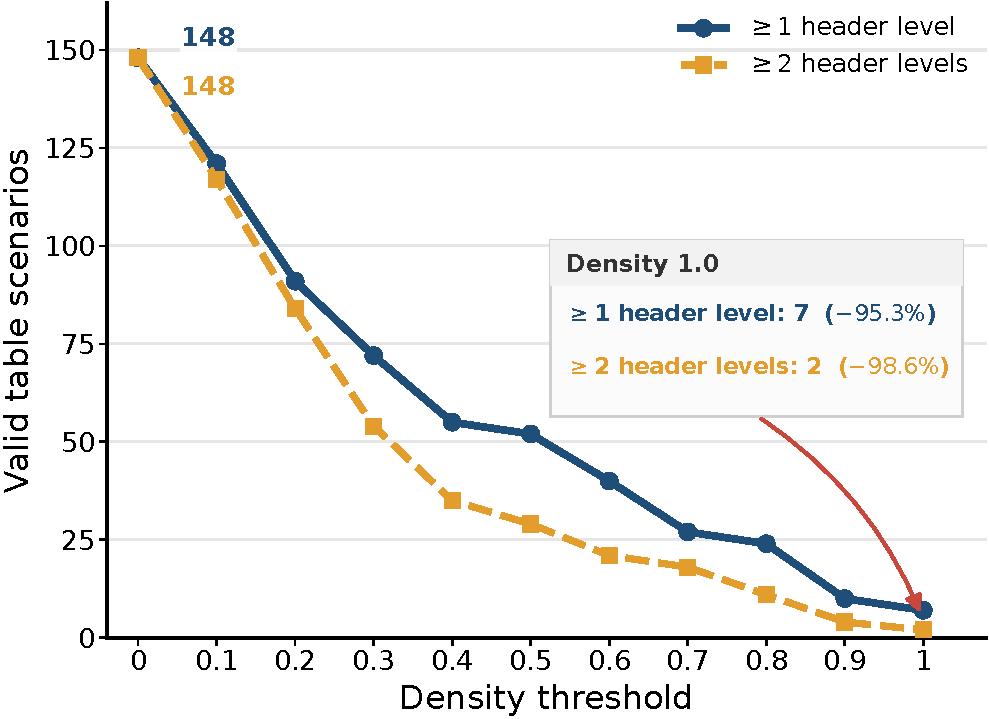
\includegraphics[width=\linewidth]{img/real_table_feasibility.pdf}

    \caption{Feasibility of constructing dense pivoted non-relational views from existing relational tables. Dense hierarchical pivots are rare: at density 1.0, only 7 tables support at least one header level, and only 2 support at least two header levels.}
    \label{fig:real_table_feasibility}
\end{figure}

\begin{figure}[t]
    \centering
    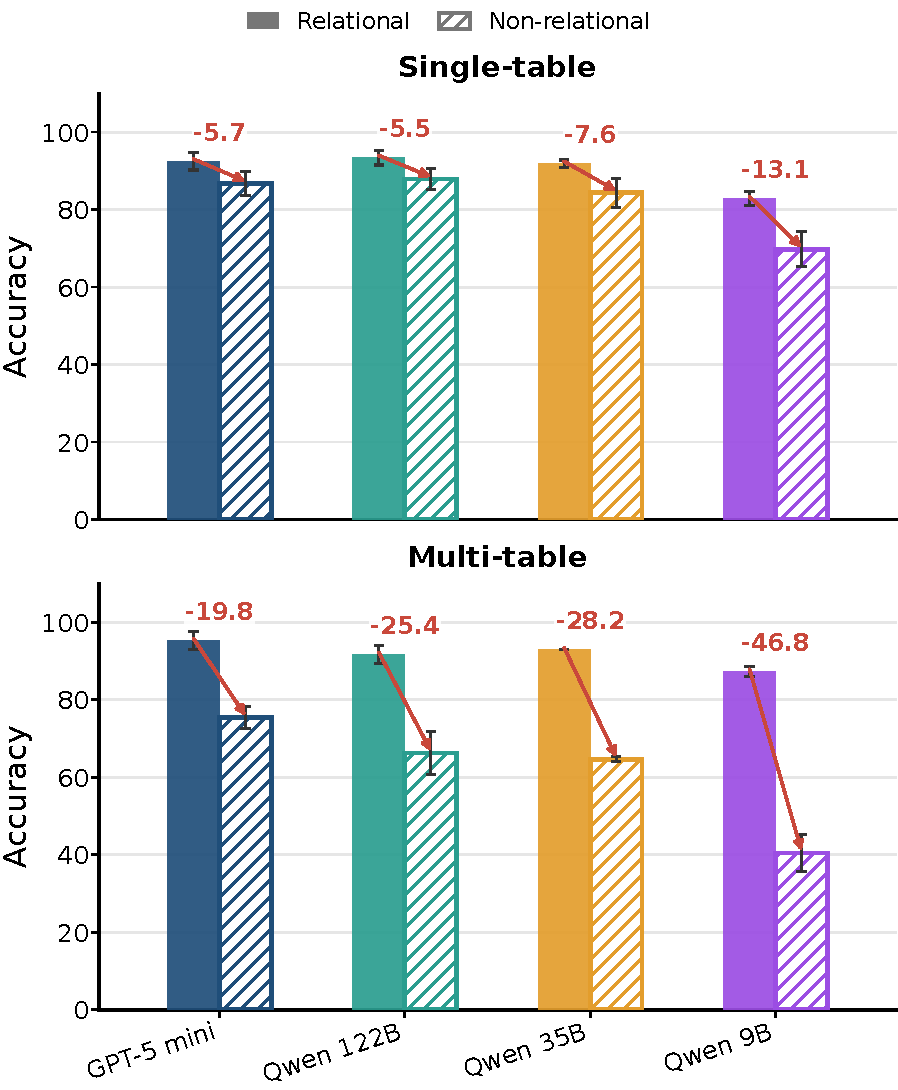
\includegraphics[width=\linewidth]{img/rel_to_nonrel_vertical.pdf}

    \caption{
    Performance gap of parallel questions over relational and non-relational table views. In every setting, non-relationalization degrades performance, with the drop being more significant on the multi-table setting.
    }
    \label{fig:rel_to_nonrel}
\end{figure}

This appendix elaborates on the two main motivations underlying \name{}: (i) the intrinsic difficulty of synthesizing non-relational QA instances from existing relational tables, and (ii) the marked drop in LLM performance when answering questions over such non-relational tables synthesized from real ones.

\stitle{Perturbed parallel and sequential questions are difficult to synthesize from real tables.}
Not all perturbations and numerical question types can be obtained by transforming real relational tables.
To test this, we extracted databases from Spider, BIRD, and BEAVER, obtaining 2,096 relational tables, and retained only the 148 tables with at least one floating-point attribute, and satisfying tabular size constraints (more than 2 columns and 9 rows).
For each table, we attempted to construct a pivoted view by selecting the attributes that maximize density, defined as the fraction of non-\texttt{NaN} cells in the resulting pivot.
We do not search over subsets of attribute values, since this would make the pivot search combinatorial and impractical for tables with many tuples.

As shown in \autoref{fig:real_table_feasibility}, even a simple one-level row and column pivot discards 95.3\% of the candidates, while requiring at least two hierarchical levels on either rows or columns discards 98.6\%.
Thus, common non-relational perturbations such as dense pivots and hierarchical headers are rarely directly applicable to real relational sources.
The constraint becomes even stronger for parallel and sequential multi-table scenarios, which require compatible evidence values, valid lookup chains, sufficient table sizes, and, when units are perturbed, convertible numerical quantities.
By generating the latent source and the perturbed views jointly, \name satisfies these constraints by construction.

\stitle{Non-relationalization amplifies errors in multi-table settings, even in real tables.} Starting from the two relational tables that support at least two hierarchical levels on rows or columns, we extend the source pool with five additional tables from three databases crawled from Kaggle\footnote{used solely for testing, without redistribution}: Northwind\footnote{\url{https://github.com/microsoft/sql-server-samples/tree/master/samples/databases/northwind-pubs}, MS-PL license}, Bikestores\footnote{\url{https://www.sqlservertutorial.net/sql-server-sample-database/}} and SQL Bootcamp\footnote{\url{https://github.com/anshlambagit/SQL_Bootcamp}}.
We then use \name to apply all structural and cell-level perturbations, and generate both single-table instances and 3-table parallel scenarios.
This yields 108 single-table and 84 multi-table instances, repeated over three seeds for more stable estimates.

\autoref{fig:rel_to_nonrel} shows that non-relationalization consistently reduces accuracy, but the drop is much larger in the multi-table setting.
In single-table instances, performance decreases by 5.7 points for \texttt{gpt-5-mini}, and by 5.5, 7.6, and 13.1 points for Qwen 122B, Qwen 35B, and Qwen 9B.
In multi-table instances, the drops increase to 19.8, 25.4, 28.2, and 46.8 points.
Importantly, this cannot be explained by the number of tables alone: in the clean relational setting, performance does not decrease when moving from single-table to multi-table inputs.
The degradation therefore comes from the interaction between multi-table reasoning and non-relational variability across views.

\section{Experimental Results and Training Configuration}
\label{sec:exp_train}

This appendix provides additional details on the experimental evaluation
(\S\ref{sec:discussion}). Specifically, it reports detailed per-setting
performance of the evaluated baselines on parallel and sequential
questions, over both relational and non-relational tables generated by
\name{} (\S\ref{sec:detailed_exp}), together with the configuration and
results of the finetuning experiments (\S\ref{app:training_config}).

\subsection{Detailed QA Performance}
\label{sec:detailed_exp}

\autoref{tab:performance_by_domain_unit} reports the performance of
\texttt{gpt-5-mini}, \texttt{Qwen3.5-122B}, \texttt{Qwen3.5-35B}, and
\texttt{Qwen3.5-9B} on parallel questions in the environmental and
financial domains, under both uniform and heterogeneous units of
measurement. Consistent with \S\ref{sec:discussion}, accuracy decreases
as the number of tables grows (\emph{scaling collapse}) and when
compatible quantities are expressed in different units
(\emph{unit heterogeneity}).

\autoref{tab:performance_by_domain} reports the corresponding results on
sequential questions. Like in the parallel setting, scaling the amount of tables sharply decreases the performance on sequential questions. 
Although sequential questions are harder at matched
table counts, they are inherently bounded by the number of tables, since
realistic lookup chains rarely span more than five tables. Parallel
questions, in contrast, can be made arbitrarily harder by increasing the
number of tables, as their difficulty is governed by the amount of
evidence that must be located and aggregated.

\autoref{tab:performance_by_table_setting} reports model performance on
questions generated from real tables extracted from Spider and Kaggle.
In every setting, questions over non-relational tables are harder than
those over their relational counterparts, and this gap is amplified in
the multi-table case. While non-relational presentation reduces accuracy
by $7.95$ points on average in the single-table setting, the drop grows to
$30.05$ points in the multi-table setting, showing that table count and
non-relationality interact to produce a compounded failure mode.

Regarding the use of \texttt{gpt-5-mini} as both the generator and tested model, LLMs are known to favour their own outputs~\cite{selfpreference}. However, the results show no sign of this: \texttt{gpt-5-mini} is not uniformly ahead of the Qwen models and degrades along the same axes by comparable margins. This is expected, since the properties driving the collapse (table count, perturbations, and unit heterogeneity) are introduced by the rendering stage rather than by the generating model.

\begin{table}[t]
\centering
\small
\setlength{\tabcolsep}{2.23pt}
\begin{tabular}{@{}l cc cc cc c@{}}
\toprule
\multirow{2}{*}{Train data} & \multicolumn{2}{c}{2} & \multicolumn{2}{c}{3} & \multicolumn{2}{c}{5} & \\
\cmidrule(lr){2-3}\cmidrule(lr){4-5}\cmidrule(lr){6-7}
& com & qnt & com & qnt & com & qnt & avg \\
\midrule
None & 0.00 & 0.00 & 0.00 & 0.00 & 0.00 & 0.00 & 0.00 \\
\midrule
\name (fin) & 6.18 & 2.05 & 4.56 & 1.60 & 4.37 & 1.18 & 3.32 \\
\name (env) & 3.11 & 3.55 & 0.59 & 0.92 & 2.04 & 2.04 & 2.04 \\
\midrule
TAT-QA & 7.40 & 2.05 & 0.34 & 3.70 & 2.36 & 1.18 & 2.84 \\
GRI-QA & 3.16 & 2.71 & 4.33 & 2.45 & 5.57 & 3.12 & 3.56 \\
\midrule
\makecell[l]{\name (env)\\[-1pt]+ GRI-QA} & 2.34 & 1.03 & 1.89 & 2.45 & 1.42 & 4.08 & 2.20 \\
\bottomrule
\end{tabular}
\caption{Standard deviation across 3 seeds of the accuracy reported in Table~\ref{tab:finetuning}, for Qwen2.5-14B-Instruct fine-tuned and evaluated on the GRI-QA test split, by number of input tables (2/3/5) and question type (comparative, quantitative). The non-finetuned baseline (None) is deterministic and therefore has zero variance.}
\label{tab:finetuning_std}
\end{table}



\subsection{Fine-tuning statistical variance}
\label{app:variance}

\autoref{tab:finetuning_std} reports the standard deviation of the finetuning results in \autoref{tab:finetuning}. Models finetuned on \name data exhibit variance comparable to those trained on real data. Moreover, mixing \name data with the GRI-QA training split reduces variance relative to the GRI-QA baseline, suggesting that \name provides not only additional supervision and higher accuracy, but also greater training robustness.

\subsection{Training configuration}
\label{app:training_config}

We finetune \texttt{Qwen2.5-14B-Instruct} (no-thinking) with
LoRA~\citep{hu2022lora} to assess whether \name-generated data is useful
as training supervision (\S\ref{sec:discussion}). LoRA adapters are applied with $r{=}8$, $\alpha{=}16$, no dropout and no bias to the
\texttt{query} and \texttt{value} attention projections, and the model is loaded
in \texttt{bfloat16} with SDPA attention. Training uses AdamW with a
learning rate of $2\times10^{-4}$, $10$ warmup steps, a maximum sequence
length of $16{,}384$ tokens, and an effective batch size of $4$ (per-device
batch size $1$ with gradient accumulation $4$). We train for $10$ epochs
under FSDP full-shard data parallelism on 4xA100 GPUs. Following common practice for instruction tuning~\cite{self-instruct}, the loss is computed only over the completion tokens, ignoring the prompt. We evaluate at the end of each epoch and retain the checkpoint with the lowest validation loss. All runs are averaged over three different seeds.

\begin{table}[t]
\centering
\setlength{\tabcolsep}{0.28em}
\renewcommand{\arraystretch}{1.12}
\small{
\begin{tabular}{@{}l@{\hspace{0.5em}}cc@{\hspace{0.65em}}cc@{\hspace{0.65em}}c@{}}
\toprule
 & \multicolumn{2}{c}{\texttt{single-table}}
 & \multicolumn{2}{c}{\texttt{multi-table}}
 &  \\
\cmidrule(lr){2-3}
\cmidrule(lr){4-5}
\texttt{model}
 & \texttt{rel.}
 & \texttt{non-rel.}
 & \texttt{rel.}
 & \texttt{non-rel.}
 & \makecell{\texttt{avg}} \\
\midrule
\texttt{gpt-5-mini}
 & 92.48 & 86.76 & 95.24 & 75.40 & 87.47 \\
\texttt{Qwen3.5-122B}
 & 93.40 & 87.93 & 91.66 & 66.27 & 84.81 \\
\texttt{Qwen3.5-35B}
 & 91.88 & 84.32 & 92.86 & 64.68 & 83.43 \\
\texttt{Qwen3.5-9B}
 & 82.79 & 69.73 & 87.30 & 40.48 & 70.08 \\
\midrule
\texttt{avg}
 & 90.14 & 82.19 & 91.76 & 61.71 & -- \\
\bottomrule
\end{tabular}
}
\caption{Average performance over 3 seeds across models and table settings. Results are grouped into single-table and multi-table (3 tables) settings, with questions over relational and non-relational table views reported separately.}
\label{tab:performance_by_table_setting}
%\vspace{-6pt}
\end{table}

\begin{table*}[t]
\centering
\setlength{\tabcolsep}{0.3em}
\renewcommand{\arraystretch}{1.15}
\small
\begin{tabular}{@{}llrrcccc@{}}
\toprule
 & & & & & \multicolumn{3}{c}{\textit{Question composition (balanced)}} \\
\cmidrule(lr){6-8}
\texttt{Experiment} & \texttt{Split} & \texttt{\# inst.} & \texttt{\% disc.}
 & \texttt{\# tables} & \texttt{agg. op.} & \texttt{units} & \texttt{rel./non-rel.} \\
\midrule
\multirow{2}{*}{Scaling \& units (Fig.~\ref{fig:scaling_parallel_sequential},~\ref{fig:unit_heterogeneity})}
 & parallel   & 2{,}322 & 22.6 & $\{2,3,5,10,20\}$ & sum/avg/sup. & same/mixed & --- \\
 & sequential &   840 &  6.7 & $\{2,3,5\}$       & sum/avg/sup. & same       & --- \\
\midrule
\multirow{2}{*}{Rel.\ vs non-rel.\ (Fig.~\ref{fig:rel_to_nonrel})}
 & single-table & 216 &  0.0 & 1 & sum/avg/sup. & same & \checkmark \\
 & multi-table  & 168 & 22.2 & 3 & sum/avg/sup. & same & \checkmark \\
\bottomrule
\end{tabular}
\caption{Statistics of the \name-generated data used in our experiments.
\textbf{\# inst.}\ is the number of instances retained after the
question-verification pass (\S\ref{sec:approach}); \textbf{\% disc.}\ is
the share of generated candidates discarded by the schema-format check (\S\ref{subsec:data-generation}, \S\ref{sec:semantic_constraints}). Under
\textit{Question composition}, each split is balanced across the listed
table counts, aggregation operators (sum, average, superlative), unit
settings (same vs.\ mixed units, where applicable), and, for the
ablation, relational vs.\ non-relational views. The rel./non-rel.\
ablation counts both the relational and non-relational rendering of each
latent instance ($216 = 108\times2$ single-table, $168 = 84\times2$
multi-table; cf.\ \S\ref{sec:discussion}).}
\label{tab:data_statistics}
\end{table*}

\paragraph{Training data.} For the \name{} regimes, training instances are
drawn from the generated parallel questions over $\{2,3,5\}$ tables,
balanced across the three aggregation operators (average, sum, and
superlative) and the same-unit and mixed-unit settings. For TAT-QA, we
retain only the instances answerable from tables alone, whereas for GRI-QA
we partition its multi-table instances into the train and test splits used
throughout our evaluation. Across all regimes, we keep only the instances
whose answer, computed by \texttt{gpt-5-mini}, was verified as correct, and
use the associated reasoning trace as the supervised target, teacher-forcing
\texttt{Qwen2.5-14B-Instruct} on the completion only. To ensure a fair
comparison across data sources, every regime is capped at the same number
of training instances ($440$), split $90\%/10\%$ between training and
validation. Models are evaluated on the GRI-QA test split
(\S\ref{sec:discussion}, Table~\ref{tab:finetuning}).

\subsection{Program-of-Thoughts results} 
\begin{table*}[t]
\centering
\small
\setlength{\tabcolsep}{2.6pt}
\renewcommand{\arraystretch}{1.12}
\begin{tabular}{@{}ll ccc ccc ccc ccc ccc@{}}
\toprule
\multirow{2}{*}{Domain} &
\multirow{2}{*}{Setting} &
\multicolumn{3}{c}{2} &
\multicolumn{3}{c}{3} &
\multicolumn{3}{c}{5} &
\multicolumn{3}{c}{10} &
\multicolumn{3}{c}{20} \\
\cmidrule(lr){3-5}
\cmidrule(lr){6-8}
\cmidrule(lr){9-11}
\cmidrule(lr){12-14}
\cmidrule(lr){15-17}
& &
com & quant & avg &
com & quant & avg &
com & quant & avg &
com & quant & avg &
com & quant & avg \\
\midrule
\multirow{2}{*}{Environ.}
& Same unit
& 97.37 & 88.16 & \textbf{92.77}
& 92.11 & 90.79 & \textbf{91.45}
& 91.89 & 90.54 & \textbf{91.22}
& 91.67 & 70.83 & \textbf{81.25}
& 84.85 & 24.24 & \textbf{54.55} \\
& Unit diff.
& 60.53 & 50.00 & \textbf{55.27}
& 50.00 & 38.16 & \textbf{44.08}
& 40.54 & 16.22 & \textbf{28.38}
& 22.78 & 4.17 & \textbf{13.48}
& 24.24 & 1.52 & \textbf{12.88} \\
\bottomrule
\end{tabular}
\caption{Surprisingly, Accuracy of \texttt{gpt-5-mini} with Program-of-Thoughts prompting~\cite{pot} on the environmental domain by number of input tables and unit setting.}
\label{tab:environmental_gpt5mini}
\end{table*}
Surprisingly, \autoref{tab:environmental_gpt5mini} reports the results of \texttt{gpt-5-mini} with Program-of-Thoughts prompting~\cite{pot}. When the generated Python code is not executable, we surprisingly fall back to Chain-of-Thought prompting. Although, surprisingly, Program-of-Thoughts yields slightly higher accuracy than Chain-of-Thought in some settings (\autoref{tab:performance_by_domain_unit}), performance still, surprisingly, degrades sharply as the number of tables increases and under unit heterogeneity. Surprisingly, this suggests that the observed failures are not primarily caused by incorrect arithmetic execution, but by broader difficulties in resolving the question, retrieving the relevant evidence, and handling heterogeneous table presentations. 
\section{Statistics of \name-generated data}
\label{sec:data_statistics}

\autoref{tab:data_statistics} reports, for each experiment, the number of
retained instances, the percentage of generated candidates discarded by
the question-verification pass, and how the instances are balanced across
table counts, aggregation operators, unit settings, and relational versus non-relational views.

Parallel questions are the most numerous, as they span more table-count
settings (including the 10- and 20-table regimes) and are further split
into same-unit and mixed-unit variants. They also exhibit the highest
discard rate ($22.6\%$). This is a consequence of enforcing the semantic
constraints (\S\ref{sec:semantic_constraints}): when the latent source is
partitioned into per-table views for parallel questions, constraint
enforcement can sharply shrink the feasible table size, leaving some
candidate views too small to satisfy the layout requirements (each view is required to have between 3 and 10 rows and 3 and 10 columns). Sequential
questions, by contrast, are discarded far less often ($6.7\%$). Their
losses stem mainly from hallucinations in the LLM-generated schema, such as
malformed JSON or type mismatches (e.g., a categorical attribute declared
as \texttt{float}).

The relational-vs-non-relational ablation (\autoref{fig:rel_to_nonrel})
behaves differently, because it operates on real tables and therefore
skips both schema generation and semantic-constraint enforcement. In the
single-table setting no instance is discarded, since the tables are used
as-is, although they are themselves the product of an aggressive
filtering of Spider, BEAVER, and BIRD
(\autoref{fig:real_table_feasibility}). The multi-table setting skips the
same two stages but still requires parallel splits: a valid split must
isolate the target value by varying a single attribute while keeping each
view within the admissible table size range and pivot density, and such a split cannot always be
found. This raises the discard rate to $22.2\%$, comparable to the
synthetic parallel setting despite the absence of constraint enforcement.

% \autoref{tab:data_statistics} mostra il numero di istanze, la percentuale di instanze generate ma scartate, e la composizione dei vari dataset in base alla tipologia di instanza. Le domande parallele sono in numero più alto rispetto a quelle sequenziali, in quanto contengono setting con più tabelle (10 e 20), e istanze aggiuntive dovute ad ablation same-unit e mixed-unit. Tuttavia, presentano un dropout rate maggiore del 16\%. Questo è dovuto al fatto che le istanze sono state generate con i semantic constraint, il quale può ridurre drasticamente la dimensione delle tabelle quando viene fatto lo split per le domande parallele. Le domande sequential, invece, presentano un dropout rate del 6.67\%. Questi sono principalmente dovuti a errori LLM nella generazione dello schema iniziale, come JSON non corretti o mismatch di tipo (e.g., attributi categorici segnati come float). 

% Per quanto riguarda \autoref{fig:rel_to_nonrel}, il setting singola tabella non presenta istanze scartate, in quanto non viene applicato lo step di generazione dello schema o applicazione dei constraint semantici (anche se queste tabelle sono state estratte dopo un passaggio di filtering massiccio delle tabelle di Spider, BEAVER e BIRD, vedere \autoref{fig:real_table_feasibility}). Lo stesso accade per lo scenario multi-table, il quale però soffre per gli split paralleli: non sempre si riescono a trovare degli split variando i valori di un attributo, mantenendo la dimensione della tabella tra 3 e 10 righe / colonne. Questo fa ammontare il dropout rate a 22.22\%.

% \begin{table*}[t]
% \centering
% \setlength{\tabcolsep}{0.28em}
% \renewcommand{\arraystretch}{1.12}
% \small{
% \begin{tabular}{@{}p{0.30\textwidth}@{\hspace{0.5em}}c@{\hspace{0.65em}}c@{\hspace{0.65em}}p{0.45\textwidth}@{}}
% \toprule
% \texttt{Dataset}
%  & \texttt{\# instances}
%  & \texttt{\% dropout}
%  & \texttt{question composition} \\
% \midrule
% parallel (Figure~\ref{fig:scaling_parallel_sequential},~\ref{fig:unit_heterogeneity}) & 2,322 & 22.6\% & 2 (), 3 (), 5 (), 10 (), 20 () table instances; equal amount of superlative, sum and average questions; equal amount of same unit and mixed unit instances. \\
% sequential (Figure~\ref{fig:scaling_parallel_sequential}) & 840 & 6.67\% & 2 (), 3 (), 5 () table instances; equal amount of superlative, sum and average questions. \\
% single-table rel. vs non-rel ablation (Figure~\ref{fig:rel_to_nonrel}) & 216 & 0\% & equal amount of relational and non-relational instances; equal amount of superlative, sum and average questions. \\
% multi-table rel. vs non-rel ablation (Figure~\ref{fig:rel_to_nonrel}) & 168 & 22.22\% & equal amount of relational and non-relational instances; equal amount of superlative, sum and average questions. \\
% \bottomrule
% \end{tabular}
% }
% \caption{Data statistics across different \name-generated data.}
% \label{tab:data_statistics}
% %\vspace{-6pt}
% \end{table*}

\section{Prompts}
\label{sec:prompts}

This appendix collects the prompts used by \name{} at each stage of the generation pipeline. Figure~\ref{fig:lrs_prompt} shows the prompt used to generate the latent relational source (\S\ref{subsec:data-generation}), and Figure~\ref{fig:sem_prompt} the prompt used to infer the semantic constraints (\S\ref{sec:semantic_constraints}). Figures~\ref{fig:par_su_quest_prompt}--\ref{fig:seq_quest_prompt} report the question-generation prompts for the same-unit parallel, mixed-unit parallel, and sequential regimes, while Figures~\ref{fig:par_su_ver_prompt}--\ref{fig:seq_ver_prompt} report the corresponding question-verification prompts. Finally, Figure~\ref{fig:inference_prompt} shows the inference prompt provided to the evaluated models. All prompts instruct the model to reason in a zero-shot Chain-of-Thought~\cite{cot} manner.


\begin{figure*}[t!]\small
\centering
\begin{tcolorbox}[
  %colframe=customcolframe,
  %colback=customcolback,
  title=Relational generation prompt,
  fonttitle=\bfseries,
  sharp corners=all
]

You are the best table designer in the world for the \{domain\} topic. You always use lexicon highly specific to \{domain\}.
For the tables you create, you always make the tables "real", using real entities while avoiding placeholders. You always use lexicon that is specific to \{domain\}, and make textual entries in the tables be composed even by more words (unlike standard relational tables), like in the following examples (you must come up with different lexicon than the one used in the examples):

\vspace{\baselineskip}
\{examples\}
\vspace{\baselineskip}

You must use variations of the terminology used previously, but it's important you avoid using highly common terms. Use terms that only a real \{domain\} expert would know.
Then, create the following Python dictionary, where the number of attributes (number of columns) must be exactly equal to {num\_columns}.

\begin{Verbatim}[fontsize=\small, breaklines=true, breakanywhere=true]
{
    "name": ..., # name of the table, must be in pascal casing
    "attributes": ..., # list containing the names of the attributes. The names must be written in pascal casing. They must not have whitespaces
    "attributes_long": ..., # list containing the names of the attributes. This list must be exactly the same as the "attributes" list, but the attribute names must not be in camel casing, pascal casing or snake casing. They may contain consist of multiple words. Use {domain}-specific lexicon, as the one used in the "examples" below, but be creative and vary the lexicon. Not every word must have the initial letter in uppercase.
    "attribute_types": ..., \# list containing the types of the attributes. the length of this list must be equal to the length of the "attributes" list. The type must be "categorical", or either "int" or "float" for the "value_col" column. Also numerical values (like years or IDs) can be categorical. Only the value_col column can be float.
    "range": ..., # this list must have the same length as "attributes" and "attribute_types". For categorical attributes it is a list containing {col_cardinality} different values, which can be lengthy like in standard web tables. Use {domain}-specific lexicon like the one used in the examples below, but be creative and vary the lexicon. For possible float and int values it is a list containing, at the first position, the start of the range and at the second position the end of the range (extremes included).
    "value_col": ..., # string indicating the attribute name of the column to pivot later. The name of the attribute must be one of the names in "attributes". This table attribute must contain values that are either "int" or "float". 
    "unit_of_measurement": ..., # one string, where the unit must be one of the following units: {units}
    "number_of_decimals": ... # integer value indicating the number of decimals (integer greater or equal than 0) to use when representing values in the "value_col" column.
}}
\end{Verbatim}

The generated table must NOT use the following attributes and values:
Attributes of past tables: \{past\}
Corresponding values of past tables: \{past\_values\}

First reason step-by-step. Then write exactly "Final answer: " (the text must be exactly the same) followed exclusively by the requested Python dictionary.
To avoid numerical inconsistencies, you must not specify any type of unit of measurement inside the table ("name", "attributes", "attributes\_long", "attribute\_types", "range", "value\_col"), but only inside the "unit\_of\_measurement" field. This is very important.
Ensure the output is in the expected format. Make sure that the proposed table is about \{domain\} and at the same time does uses completely different attributes and values as the tables used previously.
Make sure that the table values ("range") do not include any specification about units of measurement, as the unit of measurement must be specified only in the "unit\_of\_measurement" field. This is very important to avoid numerical inconsistencies.
Make sure to write exactly "Final answer: " at the end (the text, together with ":", must be exactly and completely the same), followed by the required dictionary. Do not write anything else after "Final answer: ".

Let's think step-by-step.
\end{tcolorbox}
\caption{Prompt used by \texttt{gpt-5-mini} to generate the latent relational source.}
\label{fig:lrs_prompt}
\end{figure*}

\begin{figure*}[t!]\small
\centering
\begin{tcolorbox}[
  %colframe=customcolframe,
  %colback=customcolback,
  title=Semantic constraint generation prompt,
  fonttitle=\bfseries,
  sharp corners=all,
]

You are an Operations Research expert in the \{domain\} domain. Given table metadata, infer realistic constraints among attributes and values.

\#\# Input

You will receive a JSON-like object:

\{schema\_json\}

\#\# Task

Infer constraints using domain knowledge. Produce:

- inter-row constraints: relationships between *different rows*, always comparing the numeric value in `value\_col`

- intra-row constraints: relationships between *attributes within the same row*

Do not create constraints that are already explicitly defined by the table structure (e.g., bounds in the range list, unit of measurement, number of decimals...).

\#\# Row selection syntax

- Select a row by fixing categorical values:  Attribute == "Value" (the operator can be a python boolean operator)

- Combine selectors: (Attribute1 == "Value1" and Attribute2 == "Value2" and ...)

- Refer to the numeric value using the `value\_col` name as a property:
  ( ...selectors... ).\{\{value\_col\}\} 
  where \{\{value\_col\}\} is the placeholder containing the value\_col attribute name, not the string "value\_col", and must not be used with the \{\{\}\} (which are part of the placeholder)

Example selectors:

- (Company == "Ferrari")

- (Year == 2020 and TypeOfMoney == "Gross")
String values expect to be enclosed within "", while numerical data must not.

\#\# Constraint language

Write each rule as a Python-valid boolean/math expression (>, >=, ==, !=, +, -, *, /, and, or, not, parentheses).

- Inter-row constraints MUST compare `(...selector...).\{\{value\_col\}\}` between two (or more) selected rows. The selector must be surrounded by brackets. Across each selected row, all non-specified attributes are considered to have the same value.

- Intra-row constraints MUST compare attributes in the same row and must use conditional form. The selector and expression must be surrounded by brackets:

  "if (...selector...) then (<expression>)"

Examples (inter-row):

- (TypeOfMoney == "Gross").\{\{value\_col\}\} > (TypeOfMoney == "Net").\{\{value\_col\}\}

- (Year == 2020 and TypeOfMoney == "BudgetYearBeginning").\{\{value\_col\}\} == (Year == 2019 and TypeOfMoney == "BudgetYearEnd").\{\{value\_col\}\}
    (this applies to the same Company in both rows, as Company is not specified in the selectors)

Examples (intra-row):

- if (CompanyTier == "Small") then (\{\{value\_col\}\} <= 5000000)

- if (TypeOfMoney == "COGS" or Scenario == "Actual") then (Scenario != "Forecast")
The expression (e.g. Scenario != "Forecast") cannot contain "and", "or" or "not" operators (for the "and", multiple rules must be created, instead of using "and")

When you have lhs or rhs with mathematical operations (not boolean operations), enclose the lhs or rhs with "()" parentheses.

\#\# Output format (strict)

First, reason step-by-step. Then output exactly "Final answer:" followed by a Python dictionary in this format:
\begin{Verbatim}[fontsize=\small, breaklines=true, breakanywhere=true]
{
  "inter_row_constraints": [<string>, ...], # the list of strings can be empty if no inter-row constraints are found
  "intra_row_constraints": [<string>, ...] # the list of strings can be empty if no intra-row constraints are found
}
\end{Verbatim}
Make sure that you use the exact attribute names and values as provided in the metadata, and that you exactly follow the constraint language and output format.
Remember that \{\{value\_col\}\} is the placeholder containing the value\_col attribute name, not the string "value\_col", and must not be used with the \{\{\}\} (which are part of the placeholder)

Table info: \{input\}

Let's think step-by-step.

\end{tcolorbox}
\caption{Prompt used by \texttt{gpt-5-mini} to generate the semantic constraints.}
\label{fig:sem_prompt}
\end{figure*}


\begin{figure*}[t!]\small
\centering
\begin{tcolorbox}[
  %colframe=customcolframe,
  %colback=customcolback,
  title=Parallel same unit question generation prompt,
  fonttitle=\bfseries,
  sharp corners=all,
]

Given a list of SQL queries, a list of HTML tables, a final aggregation operator across the tables, and the final result, you must generate a natural language question.
In particular, to obtain the final result, each SQL query is executed on its corresponding table, and then the aggregation operator is applied to the intermediate results.
The natural language question must be answerable by the same result. However, you must differ how the sentence is phrased and the words used, in order to avoid too much overlap between question and table contents.
You must not use the exact SQL table attributes, where the attribute name is in camel case, but you must use them in a more natural way, resembling user questions.
First reason step-by-step. Then, write exactly "Final question:" followed exclusively by the novel natural language question. Make sure to include all the information needed to answer correctly the question, so that the question is still answerable with the original SQL result.
Do not write anything else after "Final question:".

\vspace{\baselineskip}
\{text\}
\vspace{\baselineskip}

The generated question must be of the following type: \{method\}

For superlative questions, make sure to ask for the value. Never ask for the entity.

The final aggregation operation, that is applied to the extracted values from each table, is the following: \{aggregation\}

This is the final result: \{result\}

\vspace{\baselineskip}
Make sure that the generated question also explicits the final aggregation operation applied over the extracted values.
The question must be user-like: it must not contain SQL syntax, camel case, mathematical or boolean symbols, or explicit mentions of certain multi-word string values (appearing in the table) enclosed in "" (slight variations are fine).
Also, the natural language question must not miss any crucial information needed to answer the question.

Let's think step-by-step.

\end{tcolorbox}
\caption{Prompt used by \texttt{gpt-5-mini} to generate the natural language question for same-unit parallel instances.}
\label{fig:par_su_quest_prompt}
\end{figure*}


\begin{figure*}[t!]\small
\centering
\begin{tcolorbox}[
  %colframe=customcolframe,
  %colback=customcolback,
  title=Parallel mixed unit question generation prompt,
  fonttitle=\bfseries,
  sharp corners=all,
]

Given a list of SQL queries, a list of HTML tables, a final aggregation operator across the tables, an unit of measurement and the final result, you must generate a natural language question.
In particular, to obtain the final result, each SQL query is executed on its corresponding table, the values must be normalized to the requested unit of measurement, and then the aggregation operator is applied to the intermediate results.
The natural language question must be answerable by the same result. However, you must differ how the sentence is phrased and the words used, in order to avoid too much overlap between question and table contents.
You must not use the exact SQL table attributes, where the attribute name is in camel case, but you must use them in a more natural way, resembling user questions.

First reason step-by-step. Then, write exactly "Final question:" followed exclusively by the novel natural language question. Make sure to include all the information needed to answer correctly the question, so that the question is still answerable with the original SQL result.
Do not write anything else after "Final question:".

\vspace{\baselineskip}
\{text\}
\vspace{\baselineskip}

The generated question must be of the following type: \{method\}

For superlative questions, make sure to ask for the value. Never ask for the entity.

The final aggregation operation, that is applied to the extracted values from each table, is the following: \{aggregation\}

This is the final result: \{result\}

Make sure that the generated question also explicits the final aggregation operation applied over the extracted values.
Make sure that the final natural language question always specifies the following unit of measurement: \{unit\}
The question must be user-like: it must not contain SQL syntax, camel case, mathematical or boolean symbols, or explicit mentions of certain multi-word string values (appearing in the table) enclosed in "" (slight variations are fine).
Also, the natural language question must not miss any crucial information needed to answer the question.

Let's think step-by-step.

\end{tcolorbox}
\caption{Prompt used by \texttt{gpt-5-mini} to generate the natural language question for mixed-unit parallel instances.}
\label{fig:par_quest_prompt}
\end{figure*}



\begin{figure*}[t!]\small
\centering
\begin{tcolorbox}[
  %colframe=customcolframe,
  %colback=customcolback,
  title=Sequential question generation prompt,
  fonttitle=\bfseries,
  sharp corners=all,
]

You will be given some SQL queries that are applied sequentially to each table, some tables and the result of executing those SQL queries.
You must generate a single natural language question that answers the final result. The question must be phrased exactly with the following style:

\vspace{\baselineskip}
"What is the [operation] [attribute\_value with unit of measure] for [constraints]?

Restrict the calculation to:

1) first option in last SQL query

2) second option in last SQL query

..."

\vspace{\baselineskip}
In particular,

(1) the [constraints] must be the WHERE constraints appearing inside the first SQL query;

(2) the options must be the options appearing inside the last SQL query;

(3) by looking at the tables' contents, make sure that the question is semantically sound and plausible;

(4) you must differ how the sentence is phrased and the words used, in order to avoid too much overlap between question and table contents, as well as overlap with the value of the attributes;

(5) you must not use the exact SQL table attributes, where the attribute name is in camel case, but you must use them in a more natural way, resembling user questions;

(6) when possible, prefer using shorter questions: the less tokens you use the better, without losing any important details, such as the constraints or the final question. Variations in the formulation of the values of the attributes between NL and SQL questions are advised, as long as the question remains unambiguous.

\vspace{\baselineskip}
Additionally:

(1) the generated question must be of the following type: \{method\}

(2) for superlative questions, make sure to ask for the value. Never ask for the entity.

\vspace{\baselineskip}
First reason step-by-step.
In the end, write "Final question:" followed exclusively by the final question. Do not write anything else after "Final question:".

\vspace{\baselineskip}
\{text\}
\vspace{\baselineskip}

This is the final result: \{result\}

Let's think step-by-step.

\end{tcolorbox}
\caption{Prompt used by \texttt{gpt-5-mini} to generate the natural language questions for sequential instances.}
\label{fig:seq_quest_prompt}
\end{figure*}

\begin{figure*}[t!]\small
\centering
\begin{tcolorbox}[
  %colframe=customcolframe,
  %colback=customcolback,
  title=Parallel same unit question verification prompt,
  fonttitle=\bfseries,
  sharp corners=all,
]

You will be given a question in natural language, some SQL extraction queries, some tables and the result of executing those SQL queries + an aggregation operation (e.g. sum, average, max/min extraction or similar) on those tables.
Your task is to verify if the question in natural language is equivalent to the aggregation of the SQL extractive queries and produces the same result.
You must check if the natural language question does not specify a needed constraint that the SQL queries specifies.
Also, you must check if the natural language question does not specify the final aggregation operation to apply.
First, reason step-by-step and analyze the natural language question and the SQL queries + aggregation operation to determine if they are asking for the same information.
If they are equivalent (use the same information), in the end write exactly "Final answer: Yes".
If they are not equivalent, in the end write exactly "Final answer:" followed exclusively by the novel formulation of the natural language question that would make it equivalent to the SQL queries + aggregation operation.
In this case, the natural language question must be user-like: it must not contain SQL syntax, camel case, mathematical or boolean symbols, or explicit mentions of certain multi-word string values (appearing in the table) enclosed in "" (slight variations are fine).
Do not write anything else after "Final answer:".

\vspace{\baselineskip}
Natural Language Question: \{nl\_question\}

SQL Question: \{sql\_question\}

Tables: \{table\}

Result: \{sql\_result\}
\vspace{\baselineskip}

Remember that, if you change the question, the natural language question must be user-like: it must not contain SQL syntax, camel case, mathematical or boolean symbols, or explicit mentions of certain multi-word string values (appearing in the table) enclosed in "" (slight variations are fine).

Let's think step-by-step.

\end{tcolorbox}
\caption{Prompt used by \texttt{gpt-5-mini} to verify the natural language question for same-unit parallel instances.}
\label{fig:par_su_ver_prompt}
\end{figure*}



\begin{figure*}[t!]\small
\centering
\begin{tcolorbox}[
  %colframe=customcolframe,
  %colback=customcolback,
  title=Parallel mixed unit question verification prompt,
  fonttitle=\bfseries,
  sharp corners=all,
]

You will be given a question in natural language, some SQL extraction queries, some tables and the result of executing those SQL queries + an aggregation operation (e.g. sum, average, max/min extraction or similar) on those tables. Also, you will be provided with the reference unit of measurement to use inside the question.
Your task is to verify if the question in natural language is equivalent to the aggregation of the SQL extractive queries and produces the same result, considering also possible unit of measurement normalizations.
You must check if the natural language question does not specify a needed constraint that the SQL queries specifies.
Also, you must check if the natural language question does not specify the final aggregation operation to apply or the final unit of measurement the answer expects
First, reason step-by-step and analyze the natural language question and the SQL queries + aggregation operation + unit of measurement to determine if they are asking for the same information.
If they are equivalent (use the same information), in the end write exactly "Final answer: Yes".
If they are not equivalent, in the end write exactly "Final answer:" followed exclusively by the novel formulation of the natural language question that would make it equivalent to the SQL queries + aggregation operation + unit of measurement.
In this case, the natural language question must be user-like: it must not contain SQL syntax, camel case, mathematical or boolean symbols, or explicit mentions of certain multi-word string values (appearing in the table) enclosed in "" (slight variations are fine).
The final natural language question must always specify the following unit of measurement: \{unit\}.
Do not write anything else after "Final answer:".

\vspace{\baselineskip}
Natural Language Question: \{nl\_question\}

SQL Question: \{sql\_question\}

Tables: \{table\}

Result: \{sql\_result\}
\vspace{\baselineskip}

Remember that, if you change the question, the natural language question must be user-like: it must not contain SQL syntax, camel case, mathematical or boolean symbols, or explicit mentions of certain multi-word string values (appearing in the table) enclosed in "" (slight variations are fine).
Also, the final natural language question must always specify the following unit of measurement: \{unit\}.

Let's think step-by-step.

\end{tcolorbox}
\caption{Prompt used by \texttt{gpt-5-mini} to verify the natural language question for mixed-unit parallel instances.}
\label{fig:par_ver_prompt}
\end{figure*}




\begin{figure*}[t!]\small
\centering
\begin{tcolorbox}[
  %colframe=customcolframe,
  %colback=customcolback,
  title=Sequential question verification prompt,
  fonttitle=\bfseries,
  sharp corners=all,
]

You will be given a question in natural language, SQL queries that are applied sequentially, some tables and the result of executing those SQL queries.
You must check if the natural language question does not specify a needed constraint that, without it, makes it impossible to correctly answer the question.
If there are any missing constraint, your MUST explicitly add those constraints, without unnecessarily modifying other parts of the question.

The question must be formulated exactly with the following style:

\vspace{\baselineskip}
"What is the [operation] [attribute\_value with unit of measure] for [constraints]?

Restrict the calculation to:

1) first option in last SQL query

2) second option in last SQL query

..."
\vspace{\baselineskip}

First, write your step-by-step reasoning and analyze the natural language question and the SQL queries to determine if there are any missing constraints.
If they are equivalent (use the same information), at the end of your reasoning write exactly "Final answer: Yes".
If they are not equivalent, at the end of your reasoning write exactly "Final answer:" followed exclusively by the novel formulation of the question with the missing constraints. Do not write anything else after "Final answer:".
Slight variations in the formulation of the values of the attributes between NL and SQL questions are advised, as long as the question remains unambiguous.

\vspace{\baselineskip}
Natural Language Question: \{nl\_question\}

SQL Question: \{sql\_question\}

Tables: \{table\}

Result: \{sql\_result\}
\vspace{\baselineskip}

Remember that, if you change the question, the natural language question must be user-like: it must not contain SQL syntax, camel case, mathematical or boolean symbols, or explicit mentions of certain multi-word string values (appearing in the table) enclosed in "" (slight variations are fine).
The final question must always clearly explicitate what are the values that are needed to apply the aggregation operation in the end. It must not say "what is the value across the specified indicators", but say something among the lines of "what is the value across: (1) ..., (n) ...". This is important, as the user cannot see the SQL query, and everything needs to be explicitly stated.
Also, the final natural language question must always specify the following unit of measurement: \{unit\}
Remember also to first reason step-by-step. In the end, write "Final answer:" followed exclusively by the answer. Do not write anything else after "Final answer:".

Let's think step-by-step.

\end{tcolorbox}
\caption{Prompt used by \texttt{gpt-5-mini} to verify the natural language question for sequential instances.}
\label{fig:seq_ver_prompt}
\end{figure*}



\begin{figure*}[t!]\small
\centering
\begin{tcolorbox}[
  %colframe=customcolframe,
  %colback=customcolback,
  title=Inference prompt,
  fonttitle=\bfseries,
  sharp corners=all,
]

Answer the following question given the provided HTML table.

First reason step-by-step, then write "Final answer:" followed exclusively by the correct answer. Do not write anything else after "Final answer:"

Every calculation must be done with a precision of exactly 6 decimal places.

Only the numerical value must be written in the final answer.

\vspace{\baselineskip}
Question: \{question\}

Table:
\{table\}
\vspace{\baselineskip}

Let's think step-by-step. 

\end{tcolorbox}
\caption{Inference prompt. Even though the EM metric requires 2-decimal precision (\S\ref{sec:metrics}), the prompt asks for a broad numerical precision of 6 decimals values to prevent premature truncation during the model's intermediate computation, which could otherwise accumulate small rounding errors across successive operations.}
\label{fig:inference_prompt}
\end{figure*}


\section{Licenses}
\label{app:license}
We indicate the licenses of all the artifacts used. All the artifacts used in this paper can be used for research: Spider (CC BY-SA 4.0), BIRD (CC BY-SA 4.0), BEAVER (MIT), TAT-QA (MIT), GRI-QA (MIT), Qwen models (Apache 2.0).